\documentclass[12pt,a4paper]{article}
\usepackage[utf8]{inputenc}
\usepackage[francais]{babel}
\usepackage[pdftex]{graphicx}
\usepackage{amsmath}
\usepackage{amssymb}
\usepackage{float}
\usepackage{algorithm} 
\usepackage{algpseudocode}
\edef\restoreparindent{\parindent=\the\parindent\relax}
\usepackage{parskip}
\restoreparindent
\usepackage{tikz}
\usetikzlibrary{arrows, automata}
\usepackage{subcaption}
\usepackage{graphicx}

\usepackage[export]{adjustbox}
\usepackage[T1]{fontenc}
\usepackage{hyperref}
\hypersetup{
    colorlinks,
    citecolor=blue,
    filecolor=black,
    linkcolor=black,
    urlcolor=teal,
    pdftitle={Rapport de projet de master 1 - Virgil Surin},
    pdfauthor=Virgil Surin,
    pdfpagemode=FullScreen
}
\tikzset{every picture/.style={scale=1,auto=center,every node/.style={circle,fill=blue!20}}}
\graphicspath{images/}

\begin{document}

% \begin{titlepage}
%   \begin{center}

%     {\Large Université de Mons}\\[1ex]
%     {\Large Faculté des sciences}\\[1ex]
%     {\Large Département d'Informatique}\\[2.5cm]

%     \newcommand{\HRule}{\rule{\linewidth}{0.3mm}}
%     % Title
%     \HRule \\[0.3cm]
%     { \LARGE \bfseries Étude comparative d'algorithmes pour énumérer les cliques d'un graphe \\[0.3cm]}
%     % { \LARGE \bfseries Rapport préliminaire de projet de Master \\[0.1cm]} % Commenter si pas besoin
%     \HRule \\[1.5cm]

%     % Author and supervisor
%     \begin{minipage}[t]{0.45\textwidth}
%       \begin{flushleft} \large
%         \emph{Directeur:}\\
%         Hadrien \textsc{Mélot}\\
%         \emph{Co-directeur:}\\
%         Sébastien \textsc{Bonte}\\
%       \end{flushleft}
%     \end{minipage}
%     \begin{minipage}[t]{0.45\textwidth}
%       \begin{flushright} \large
%         \emph{Auteur:} \\
%         Virgil \textsc{Surin}
%       \end{flushright}
%     \end{minipage}\\[2ex]

%     \vfill

%     % Bottom of the page
%     \begin{center}
%       \begin{tabular}[t]{c c c}
%         
\includegraphics[height=1.5cm]{logoumons.jpg} &
%                                                         \hspace{0.3cm} &
%                                                                          
\includegraphics[height=1.5cm]{logofs.jpg}
%       \end{tabular}
%     \end{center}~\\

%     {\large Année académique 2023-2024}

%   \end{center}
% \end{titlepage}
\begin{titlepage}
  \begin{center}
    \textnormal{\Large{Universit\'e de Mons}}\\[0.3em]
    \textnormal{\Large{Facult\'e des Sciences}}\\[0.3em]
  \end{center}
  \vspace*{3cm}
  \begin{center}
    \fbox{
      \begin{minipage}{0.9\textwidth}
        \centering
        \vspace*{0.5cm}\textbf{\LARGE{Étude comparative d'algorithmes\\}}
        \textbf{\LARGE{d'énumération de cliques d'un graphe }}\vspace*{0.5cm}
      \end{minipage}
    }
  \end{center}
  \vspace*{2cm}

  \begin{minipage}[t]{0.45\textwidth}
    \begin{flushleft} \large
      \emph{Directeur:}\\
      Hadrien \textsc{Mélot}\\
      \emph{Co-directeur:}\\
      Sébastien \textsc{Bonte}\\
    \end{flushleft}
  \end{minipage}
  \begin{minipage}[t]{0.45\textwidth}
    \begin{flushright} \large
      \emph{Auteur:} \\
      Virgil \textsc{Surin} \\
    \end{flushright}
  \end{minipage}\\[2ex]

  \vspace*{2cm}
  \begin{center}
    
\includegraphics[height=1.7cm]{images/logoumons.jpg}
    \hspace{1cm}
    
\includegraphics[height=1.7cm]{images/logofs.jpg}
    \\[1em]
    Ann\'ee acad\'emique 2023-2024
  \end{center}

\end{titlepage}

\tableofcontents

\newpage

\section{Introduction}


Dans ce rapport nous allons étudier plusieurs algorithmes d'énumeration de cliques maximales dans un graphe simple non orienté. Cette étude se base principalement sur l'article d'Alessio Conte et Etsuji Tomita  \textit{''On the overall and delay complexity of the CLIQUES and Bron-Kerbosch algorithms''} \cite{CONTE20221}.

L'objectif de ce projet est d'implémenter les algorithmes présentés et de confirmer les résultats obtenus par M.Conte et M.Tomita. Également, ces algorithmes seront implémentés en Python et en Rust afin de valider le gain de temps de Rust par rapport à Python.

Nous commencerons par un rappel des notions et notations utilisées ainsi que des définitions utiles à la compréhension de ce rapport, suivi d'une présentation des différents algorithmes implémentés et pour terminer par la comparaison d'efficacité en temps et en langage de ceux-ci.

\section{Les cliques, cas d'utilisations}%
\label{sec:usecase}

Étudier le problème d'énumération de cliques maximales et développer des algorithmes efficaces pour ce faire présente un intérêt considérable en raison de la multitude de systèmes qui peuvent être modélisés par des graphes. Dans de nombreux contextes, des amats de sommets tous connectés entre eux, connus sous le nom de cliques, apparaissent naturellement. Ces cliques peuvent représenter des compartiments indépendants ou des unités logiques au sein du système étudié.

Les applications des cliques sont variées et couvrent de nombreux domaines. En biologie, par exemple, les cliques peuvent représenter des complexes protéiques où chaque protéine interagit avec toutes les autres du complexe, fournissant ainsi des informations cruciales pour comprendre les réseaux de signalisation cellulaire et les interactions protéine-protéine \cite{PAVLOU2016305}.

Dans le domaine de la sociologie, les cliques sont utilisées pour identifier des groupes d'individus ayant des interactions fréquentes et intenses, ce qui peut aider à analyser les structures sociales et les dynamiques de groupe \cite{SCOTT201129}.

En informatique, les cliques peuvent être utilisées dans l'optimisation des requêtes de bases de données et dans la détection de communautés au sein des réseaux de communication \cite{CORMEN200932}.

En résumé, la capacité à identifier efficacement les cliques dans un graphe a des applications concrètes, allant de la compréhension des systèmes biologiques complexes à l'analyse des structures sociales en passant par l'optimisation des systèmes informatiques. Ces exemples illustrent l'importance pratique des cliques dans la recherche et les applications réelles\cite{FORTUNATO201075}.

\section{Les graphes}%
\label{sec:graphes}

\subsection{Notions de bases}

Dans ce rapport, nous allons définir un graphe simple non orienté \emph{G=V, E} comme étant un ensemble de nœuds \emph{V} reliés par des arêtes. Nous notons l'ensemble des arêtes comme étant l'ensemble \emph{E}. Une arêtes est définie comme un tuple $ (v, v') $ où $ v $ et $ v' $ sont les 2 nœuds réliés par l'arête. Les nœuds peuvent être étiquetés pour plus de lisibilité.


Nous considérons des graphes simples non dirigés, c'est à dire qu'il y a au plus une et une seule arête entre deux nœuds et aucune arête allant d'un nœud à lui-même. Les arêtes que nous considérons n'ont pas de sens particulier. Ainsi, l'arête joignant les nœuds \emph{x} et \emph{y} est la même que celle joignant \emph{y} à \emph{x} et sera dénotée par l'existence du tuple $(x, y) \in E$.

L'ordre \emph{n} d'un graphe est défini comme étant $ |V| $ et sa taille \emph{m} comme $ |E| $.

Dans la Figure \ref{fig:x exemple1}, nous pouvons observer un premier graphe \textit{a} dont l'ensemble des noeuds \(V\) est l'ensemble \(\{1, 2, 3\}\). L'ensemle des arretes \(E\) quant a lui est l'ensemble \(\{(1,2), (2,3)\}\). Le graphe \textit{a} est un graphe d'ordre 3 et de taille 2. De la meme facon, pour le graphe \textit{b} on a \(V = \{1, 2, 3, 4, 5\}\) et \(E = \{(1,2), (2,3), (4,5)\}\). \textit{b} est d'ordre 5 et de taille 3.

\begin{figure}[h]
  \begin{subfigure}[b]{0.50\textwidth}
    \centering
        \begin{tikzpicture}

          \node (v1) at (0, 0){1};
          \node (v2) at (0, 2){2};
          \node (v3) at (2, 2){3};

          \draw[-](v1)--(v2);
          \draw[-](v2)--(v3);

        \end{tikzpicture}
        \caption{}
        \label{fig:x g1}
  \end{subfigure}
  \begin{subfigure}[b]{0.50\textwidth}
    \centering
        \begin{tikzpicture}

          \node (v1) at (0, 0){1};
          \node (v2) at (1, 2){2};
          \node (v3) at (3, 2){3};
          \node (v4) at (2, 0){4};
          \node (v5) at (4, 1){5};

          \draw[-](v1)--(v2);
          \draw[-](v2)--(v3);
          \draw[-](v4)--(v5);

        \end{tikzpicture}
        \caption{}
        \label{fig:x g2}
  \end{subfigure}
  \caption{Deux graphes}
  \label{fig:x exemple1}
\end{figure}

Soit \emph{G=V, E} Nous définirons les voisins d'un noeud \emph{v} comme l'ensemble des noeuds directement relié à \emph{v} par une arrete. Nous noterons l'ensemble des voisins de \emph{v} comme \emph{N(v)} définit formellement comme suit:
\begin{equation}
N(v) = { v' | (v, v') \in E }
\end{equation}
Prenons le noeud \emph{2} du graphe \emph{b} de la Figure \ref{fig:x exemple1}. L'ensemble des voisins de ce noeud est l'ensemble \(N = {1, 3}\).


Soit \emph{G = V, E}, un sous-graphe induit de \emph{G}, noté \(SG = W, E(W)\), est un graphe construit à partir d'un sous-ensemble de noeud de \emph{V} où $ W \subseteq V $ et $ E(W) = E \cap (W \times W) $. Nous appellons \emph{SG=W, E(W)}..
Notez que dans un sous-graphe induit, nous ne conservons pas les arrêtes dont une extrémité ne se trouve pas dans \emph{W}.

Par exemple, en prenant le graphe \textit{b} de la Figure \ref{fig:x exemple1}, le sous-graphe \(SG=\{1, 2, 5\}, E(\{1, 2, 5\})\) est un sous-graphe valide de \textit{b} contenant uniquement les noeuds 1, 2 et 5 (\(W\)) et l'arrete \((1,2)\) (\(E(W)\)).

\begin{figure}
  \centering
  \begin{tikzpicture}

    \node (v1) at (0, 0){1};
    \node (v2) at (1, 2){2};
    \node (v5) at (4, 1){5};

    \draw[-](v1)--(v2);

  \end{tikzpicture}
  \caption{un sous-graphe de \textit{b}}
\end{figure}

\subsection{Les cliques}%
\label{subsec:cliques}

Une \textit{clique} est définie comme suit :
soit un graphe \emph{G=V,E}. Nous dirons que \(C \subseteq V\), un sous-ensemble de noeuds du graphe, est une clique si et seulement si tous les noeuds de \emph{C} sont voisins entre-eux.
C'est-à-dire :
\begin{equation}\label{clique}
\forall v, w \in C \ | \ (v, w)\in E \ avec\  v \neq w
\end{equation}

\begin{figure}[h]
  \centering
  \begin{tikzpicture}

    \node[fill=red!20](v1) at (0, 0){1};
    \node[fill=red!20](v2) at (0, 2){2};
    \node[fill=red!20](v3) at (2, 2){3};
    \node[fill=red!20](v4) at (3, 0){4};
    \node (v5) at (4, 2){5};
    \node (v6) at (6, 1.5){6};
    \node (v7) at (5, 0){7};

    \draw[red!20, ultra thick](v1)--(v2);
    \draw[red!20, ultra thick](v2)--(v3);
    \draw[red!20, ultra thick](v1)--(v3);
    \draw[red!20, ultra thick](v1)--(v4);
    \draw[red!20, ultra thick](v2)--(v4);
    \draw[red!20, ultra thick](v3)--(v4);
    \draw[-](v3)--(v5);
    \draw[-](v4)--(v5);
    \draw[-](v5)--(v6);
    \draw[-](v4)--(v6);
    \draw[-](v4)--(v7);
    \draw[-](v6)--(v7);
  \end{tikzpicture}
  \caption{Un graphe, en rouge une clique de ce graphe}
  \label{fig:x clique1}
\end{figure}

Il est important de remarquer qu'avec cette définition d'une clique, un noeud seul n'est pas une clique.

La \textit{taille} d'une clique est définie par sa cardinalité, c'est à dire que la taille d'une clique \emph{C} est \(|C|\). Comme exemple, prenons la clique en rouge dans le graphe de la Figure \ref{fig:x clique1} : nous avons que \(C = \{1,2,3,4\}\) et \(|C| = 4\). C'est donc une clique de taille 4.

Nous dirons qu'une clique est \textit{maximale} s'il est impossible de rajouter un nœuds de \emph{G} dans la clique tel que la propriété \eqref{clique} reste respectée.

Dans la Figure \ref{fig:x clique1}, la clique \textit{bleue} composée des noeuds 1, 2, 3 et 4 est egalement maximale. Par contre, la clique composée des noeuds 3 et 5 ne l'est pas car il est possible d'y rajouter le noeud 4.

Enfin, nous définirons une clique \textit{maximum} comme étant une clique de taille maximum. Notons que toute clique maximum sera maximale et qu'il peut y avoir plusieurs cliques maximum dans un même graphe.

\begin{figure}[h]
  \begin{center}
\begin{tikzpicture}

  \node (v1) at (0, 0){1};
  \node (v2) at (0, 2){2};
  \node[fill=red!20](v3) at (2, 2){3};
  \node[fill=red!20](v4) at (3, 0){4};
  \node[fill=red!20](v5) at (4, 2){5};
  \node (v6) at (6, 1){6};
  
  \draw[-](v1)--(v2);
  \draw[-](v2)--(v3);
  \draw[red!20, ultra thick](v3)--(v4);
  \draw[red!20, ultra thick](v3)--(v5);
  \draw[red!20, ultra thick](v4)--(v5);
  \draw[-](v5)--(v6);
\end{tikzpicture}
\caption{Un graphe}
  \label{fig:x clique2}
\end{center}
\end{figure}

Regardons la Figure \ref{fig:x clique2}. $ \{3, 4, 5\}$ (en rouge) est une clique maximale et maximum car il n'est pas possible de rajouter un noeud à cette clique tel qu'il sera voisin de 3, 4 et 5 (maximale) et il n'existe pas de clique de plus grande taille (maximum). Par contre, la clique composée des noéuds 1 et 2, bien qu'étant maximale (en effet, aucun autre noeud du graphe ne peut être ajouté à cette clique) n'est pas maximum car elle ne contient que 2 noeuds là où la clique précédemment mentionnée (celle en rouge sur la figure \ref{fig:x clique2}) est plus grande vu qu'elle contient 3 noeuds.

\subsection{Quelques types de graphes}%
\label{subsec:graphes}

\subsubsection*{Graphe complet}
\label{subsubsec:complet}

Un graphe complet d'ordre \emph{n} est un graphe avec le maximum d'arrêtes possibles, c'est à dire \(\frac{n(n-1)}{2}\) arrêtes. Dans un graphe complet, chaque noeud est directement connectés à chaque noeuds, autrement dit, le graphe \(G = V, E\) est complet si et seulement si on a :
\begin{equation}
\forall (v,w) \in V \ | \ (v, w) \in E \ \text{avec} \ v \neq w
\end{equation}

La Figure \ref{fig:k6} représente un graphe complet d'ordre 6.

\begin{figure}[h!]
    \centering
    \begin{tikzpicture}
        % Define the positions of the nodes
        \node (n1) at (0, 0) {1};
        \node (n2) at (3, 0) {2};
        \node (n3) at (-2, 2) {3};
        \node (n4) at (5, 2) {4};
        \node (n5) at (0, 4) {5};
        \node (n6) at (3, 4) {6};

        % Draw the edges
        \foreach \from/\to in {
          n1/n2, n1/n3, n1/n4, n1/n5, n1/n6,
          n2/n3, n2/n4, n2/n5, n2/n6,
          n3/n4, n3/n5, n3/n6,
          n4/n5, n4/n6,
          n5/n6,
        }
        \draw (\from) -- (\to);
    \end{tikzpicture}
    \caption{Graphe complet d'ordre 6}
    \label{fig:k6}
\end{figure}

Il est évident qu'un graphe complet contient une et une seule clique maximale (qui est donc également maximum) et que celle-ci est de taille \emph{n}. Il s'agit de l'ensemble du graphe.

\subsubsection*{Graphe vide}
\label{subsubsec:vide}

Un graphe vide d'ordre \emph{n} est un graphe ne possédant aucune arrête. C'est-à-dire dont la taille \emph{m} est égale à 0. Un exemple de graphe vide d'ordre 4 est donné ci-dessous (Figure \ref{fig:vide}).
Naturellement, un graphe vide d'ordre \emph{n} possède \emph{n} cliques maximales de tailles 1 et elles sont toutes maximum.

\begin{figure}[h!]
  \centering
  \begin{tikzpicture}
    \node (n1) at (0, 0) {1};
    \node (n2) at (2, 0) {2};
    \node (n3) at (0, 2) {3};
    \node (n4) at (2, 2) {4};

    \foreach \from/\to in {
    }
    \draw (\from) -- (\to);
  \end{tikzpicture}
  \caption{Graphe vide d'ordre 4}
  \label{fig:vide}
\end{figure}

\subsubsection*{Graphe de Turàn}
\label{subsubsec:turan}

Un graphe de Turán, noté \( T(n, r) \), est un graphe formé en partitionnant un ensemble de \( n \) sommets en \( r \) sous-ensembles aussi égaux que possible, et en connectant deux sommets par une arête si et seulement s'ils appartiennent à des sous-ensembles différents. Les graphes de Turán sont souvent utilisés dans la théorie des graphes extrémaux car ils maximisent le nombre d'arêtes sans contenir un certain sous-graphe interdit, comme un \( K_{r+1} \) (le graphe complet sur \( r+1 \) sommets).

Formellement, le graphe de Turán \( T(n, r) \) est défini comme suit :
\begin{itemize}
  \item Partitionner les \( n \) sommets en \( r \) sous-ensembles \( V_1, V_2, \ldots, V_r \) aussi égaux que possible.
  \item Ajouter une arête entre deux sommets \( u \) et \( v \) si et seulement s'ils appartiennent à des sous-ensembles différents, c'est-à-dire \( u \in V_i \) et \( v \in V_j \) avec \( i \neq j \).
\end{itemize}

Considérons \( T(9, 3) \) (Figure \ref{fig:turan}). Nous partitionnons les 9 sommets en 3 sous-ensembles de 3 sommets chacun. Les arêtes connectent les sommets de sous-ensembles différents.

\begin{figure}[h!]
  \centering
  \begin{tikzpicture}

    \node[fill=green!50] (n1) at (0, 0) {1};
    \node[fill=green!50] (n2) at (2, 0) {2};
    \node[fill=green!50] (n3) at (4, 0) {3};

    \node[fill=blue!50] (n4) at (-2, 1) {4};
    \node[fill=blue!50] (n5) at (-2, 3) {5};
    \node[fill=blue!50] (n6) at (-2, 5) {6};

    \node[fill=red!50] (n7) at (0, 6) {7};
    \node[fill=red!50] (n8) at (2, 6) {8};
    \node[fill=red!50] (n9) at (4, 6) {9};

    \foreach \from/\to in {
      n1/n4, n1/n5, n1/n6, n1/n7, n1/n8, n1/n9,
      n2/n4, n2/n5, n2/n6, n2/n7, n2/n8, n2/n9,
      n3/n4, n3/n5, n3/n6, n3/n7, n3/n8, n3/n9,
      n4/n7, n4/n8, n4/n9,
      n5/n7, n5/n8, n5/n9,
      n6/n7, n6/n8, n6/n9
    }
    \draw (\from) -- (\to);
  \end{tikzpicture}
  \caption{Graphe de Turán \( T(9, 3) \)}
  \label{fig:turan}
\end{figure}

Dans cet exemple, les sommets \{1, 2, 3\}, \{4, 5, 6\}, et \{7, 8, 9\} forment les trois sous-ensembles. Chaque sommet est connecté à tous les sommets des autres sous-ensembles, mais il n'y a pas d'arêtes entre les sommets d'un même sous-ensemble.

\subsubsection*{Graphes de Moon-Moser}
\label{subsubsec:mm}

Les graphes de Moon-Moser sont un sous-ensemble particulier de graphes de Turán. Un graphe de Moon-Moser est un graphe \( T(n, \lceil n/3 \rceil) \).

Considérons un graphe de Moon-Moser avec 6 sommets, c'est-à-dire \( T(6, 2) \). Nous avons deux sous-ensembles de trois sommets chacun, et chaque sommet est connecté à tous les sommets des autres sous-ensembles.

\begin{figure}[h!]
    \centering
    \begin{tikzpicture}
        \node (n1) at (0, 0) {1};
        \node (n2) at (3, 0) {2};
        \node (n3) at (6, 0) {3};
        \node (n4) at (0, 3) {4};
        \node (n5) at (3, 3) {5};
        \node (n6) at (6, 3) {6};

        \foreach \from/\to in {
          n1/n4, n1/n5, n1/n6,
          n2/n4, n2/n5, n2/n6,
          n3/n4, n3/n5, n3/n6}
        \draw (\from) -- (\to);
    \end{tikzpicture}
    \caption{Graphe de Moon-Moser d'ordre 6}
    \label{fig:moon-moser}
\end{figure}

Dans cet exemple, les deux sous-ensembles sont \{1, 2, 3\} et \{4, 5, 6\}. Chaque sommet est connecté à tous les sommets de l'autre sous-ensemble.

Les graphes de Moon-Moser maximisent le nombre de cliques maximales dans un graphe \cite{MR0182577}.

\section{Le problème d'énumération des cliques dans un graphe}

\subsection{Définition}%
\label{subsec:def_prob}

Ce problème consiste, dans un graphe simple, à énumérer toutes les cliques \textbf{maximales} de celui-ci. L'ordre dans lequel celles-ci sont listées n'est pas important.

\begin{figure}[h]
  \begin{center}
    \begin{tikzpicture}

      \node (v1) at (0, 1){1};
      \node (v2) at (0, 3){2};
      \node (v3) at (2, 2){3};
      \node (v4) at (4, 0){4};
      \node (v5) at (4, 2){5};
      \node (v6) at (6, 3){6};
      \node (v7) at (6, 1){7};

      \draw[-](v1)--(v2);
      \draw[-](v1)--(v3);
      \draw[-](v2)--(v3);
      \draw[-](v3)--(v4);
      \draw[-](v3)--(v5);
      \draw[-](v4)--(v5);
      \draw[-](v5)--(v6);
      \draw[-](v5)--(v7);
      \draw[-](v4)--(v7);
      \draw[-](v4)--(v6);
      \draw[-](v6)--(v7);
    \end{tikzpicture}
    \caption{}
    \label{fig:x clique3}
  \end{center}
\end{figure}


Prenons par exemple le graphe en Figure \ref{fig:x clique3}. Nous sommes donc intéressé d'obtenir les cliques suivantes :
\begin{itemize}
        \item \(\{1, 2, 3\}\)
        \item \(\{5, 4, 3\}\)
        \item \(\{4, 5, 7, 6\}\)
\end{itemize}
Ces trois cliques sont bien les seules et uniques cliques maximales de ce graphe. De plus, la clique maximum est celles contenant les noeuds 4, 5, 6 et 7.
Notez comme la clique \({4, 5, 6}\) n'est pas reprise, en effet celle-ci n'est pas maximale car elle peut être agrandie avec le noeud 7.

\subsection{Complexité du problème}
L'énumération des cliques maximales dans un graphe simple est un problème fondamental en théorie des graphes et en informatique théorique. Ce problème consiste à identifier toutes les cliques maximales d'un graphe, c'est-à-dire les sous-graphes complets qui ne peuvent être étendus par l'ajout d'un sommet adjacent. Bien que le problème soit simple à énoncer, sa complexité algorithmique est élevée et pose des défis importants. Ce problème est un problème \(\mathcal{N}\mathcal{P}\text{-Difficile}\).

Le nombre de cliques maximales dans un graphe peut être exponentiel par rapport au nombre de sommets du graphe. En effet, Moon et Moser ont démontré qu'un graphe simple à \(n\) noeuds a au plus \( 3^{n/3} \) cliques maximales\cite{MR0182577}. D'ailleurs, les graphes qui maximise le nombre de cliques maximales sont nommés graphe de Moon-Moser (voir section \ref{subsubsec:mm}).

Nous allons ici présenter un algorithme (et des variantes) qui atteint une complexité dans le pire des cas de \(O(3^{3/n})\)\cite{CONTE20221}, correspondant ainsi au nombre de cliques qu'il faut énumérer (dans le pire des cas). Même si ce résultat semble décevant, il signifie surtout que nous pouvons énumérer toutes les cliques en temps polynomial par rapport au nombre de cliques dans le graphe. Cela implique que le délai pour trouver la prochaine clique est également polynomial. En pratique, cet algorithme et ces variantes se comportent plutôt bien en terme de temps.

\section{Idée générale}%
\label{sec:idee}

\subsection{Explication}%
\label{subsec:explication}

Dans cette section nous allons aborder et expliquer l'idée générale commune à chacun des algorithmes présentés dans les sections \ref{sec:clique} et \ref{sec:bk1}.

Rappellons que l'objectif de ces algorithmes est d'énumérer toutes les cliques maximales dans un graphe \emph{G = (V, E)}.

L'idée est de passer par une recherche en profondeur. L'algorithme commence avec un ensemble de tous les sommets du graphe et explore récursivement toutes les combinaisons possibles de sommets pour former des cliques en appliquant des techniques d'élagages afin de ne pas considérer de duplicata.

Pour ce faire, notre procédure défini trois ensembles de sommets :
\begin{itemize}
  \item \emph{Q}, la clique en train d'être énumérée
  \item \texttt{SUBG}, qui représente les sommets restants à explorer (notez que \texttt{SUBG} est un sous-graphe induit de \emph{G}).
  \item \texttt{CAND}, qui contient les sommets qui peuvent être ajoutés à \emph{Q} (les candidats). \texttt{CAND} est entièrement contenue dans \texttt{SUBG}.
\end{itemize}
À chaque étape de la recherche, un sommet \emph{p} est sélectionné et ajouté à \emph{Q}.  Ensuite, nous réduisons \texttt{SUBG} à \texttt{SUBG} \(\cap\) \emph{N(p)} et \texttt{CAND} à \texttt{CAND} \(\cap\) \emph{N(p)}. Lorsque nous remontons dans la recherches (backtracking), nous retirons \emph{p} des \texttt{CAND}idats mais pas de \texttt{SUBG}. Ainsi les cliques contenues dans \texttt{CAND} n'auront pas de doublons (vu que nous ne cherchons que les maximales, lorsque nous trouvons une clique maximale avec \emph{p} il n'est pas nécessaire de chercher une autre clique maximale contenant \emph{p} car elles ont déjà toutes été trouvées lors de l'exploration des cliques contenant \emph{p})

Lorsque \texttt{SUBG} est vide, cela veut dire que nous avons trouvé une clique maximale car il n'y a plus de sommet à explorer.

\subsection{Le pivotage}%
\label{subsec:pivotage}


Afin d'optimiser la recherche en profondeur nous choisissons, avant de choisir un sommet \emph{p}, un noeud pivot \emph{u} qui permettra d'élaguer la recherche. Car chaque clique maximale \emph{Q'} dans \texttt{SUBG} \(\cap\) \emph{N(u)} n'est en réalité pas maximale dans \texttt{SUBG} vu que \emph{Q'} \(\cup \{u\}\) est une clique plus grande dans \texttt{SUBG}. Ainsi nous pouvons couper l'exploration de tous les sommets dans \emph{N(u)}.


La stratégie de pivot est une technique utilisée pour réduire le nombre de récursions nécessaires en sélectionnant un sommet pivot et en explorant ses voisins. Voici comment cette stratégie fonctionne :

L'algorithme commence par sélectionner un pivot, noté \( u \), dans \texttt{SUBG}. Nous discuterons de plusieurs stratégies pour choisir ce pivot plus tard.

Une clique maximale \( Q' \) dans \(\texttt{SUBG} \cap N(u)\) n'est pas maximale dans \( \texttt{SUBG} \), car \( Q' \cup \{u\} \) est une clique plus grande dans \( \texttt{SUBG} \) étant donné que tous les sommets de \(Q'\) sont voisins de \emph{u}. Ainsi, toute clique maximale contient soit \( u \), soit au moins un sommet de \( \texttt{SUBG} \setminus N(u) \). Cela signifie que nous pouvons ignorer l'expansion de tous les sommets dans \( N(u) \) et n'explorer que ceux dans \( \texttt{SUBG} \setminus N(u) \).

Voici un exemple détaillé.

\begin{figure}[h!]
    \centering
    \begin{subfigure}[b]{0.45\textwidth}
        \centering
        \begin{tikzpicture}
            \node (n1) at (0, 0) {1};
            \node (n2) at (0, 2) {2};
            \node (n3) at (2, 2) {3};
            \node (n4) at (3, 0) {4};
            \node (n5) at (4, 2) {5};
            \node (n6) at (4, 0) {6};
            \node (n7) at (5, 1) {7};

            \foreach \from/\to in {n1/n2, n2/n3, n1/n3, n1/n4, n3/n4, n3/n5, n4/n5, n4/n6, n5/n6, n5/n7}
              \draw (\from) -- (\to);
        \end{tikzpicture}
        \caption{SUBG}
        \label{fig:initial}
    \end{subfigure}
    \hfill
    \begin{subfigure}[b]{0.45\textwidth}
        \centering
        \begin{tikzpicture}
            \node (n1) at (0, 0) {1};
            \node (n2) at (0, 2) {2};
            \node (n3) at (2, 2) {3};
            \node (n4) at (3, 0) {4};
            \node (n5) at (4, 2) {5};
            \node (n6) at (4, 0) {6};
            \node (n7) at (5, 1) {7};

            \foreach \from/\to in {n1/n2, n2/n3}
              \draw[red!20, ultra thick] (\from) -- (\to);
            \foreach \from/\to in {n3/n5, n4/n5, n1/n3, n1/n4, n3/n4, n5/n6, n4/n6, n5/n7}
              \draw (\from) -- (\to);
            \node[fill=red!20] at (0, 2) {2};
        \end{tikzpicture}
        \caption{Sélection du pivot (2)}
        \label{fig:pivot}
    \end{subfigure}
    \vfill
    \begin{subfigure}[b]{0.5\textwidth}
        \centering
        \begin{tikzpicture}
            \node (n4) at (0, 0) {4};
            \node (n5) at (1, 2) {5};
            \node (n6) at (1, 0) {6};
            \node (n7) at (2, 1) {7};
            \foreach \from/\to in {n4/n5, n5/n6, n4/n6, n5/n7}
              \draw (\from) -- (\to);
        \end{tikzpicture}
        \caption{\(\texttt{SUBG} \backslash N(u)\) }
        \label{fig:subgraph1}
    \end{subfigure}
    \caption{Étapes de l'algorithme d'énumération des cliques maximales avec pivot}
    \label{fig:cliques_algorithm}
\end{figure}

L'algorithme commence par sélectionner un pivot. Supposons que nous choisissons le sommet 2.
Clairement, toute clique maximale dans \(\texttt{SUBG} \cap N(u)\) ne sera pas maximale si l'on tient en compte le noeud \emph{u}.

L'utilisation d'un pivot est cruciale car elle permet de réduire le nombre d'appel récursif.

\subsection{Pseudo-code commun}%
\label{subsec:algo}

Ci-dessous ce trouve le pseudo code générique des différents algorithmes que nous présentons. Il s'agit là de leur squelette commun. La partie sur le choix du pivot est volontairement laissée floue et sera précisée dans les sous-sections respectives de chacun des algorithmes.

\begin{algorithm}[H]
  \textbf{Input}: un graphe $G = (V,E)$

  \textbf{Output}: toutes les cliques maximales de $G$
  \begin{algorithmic}[1]
    \Procedure{ALG}{$SUBG, CAND$}
      \If{$SUBG = \emptyset$} \Comment{$Q$ est une clique maximale}
        \State \textbf{print} ($ Q $)
      \Else
        \State $u \gets$ un noeud pivot de \emph{SUBG}
        \While{ il reste des noeuds candidats}
          \State $p \gets$ un noeud dans $CAND \setminus N(u)$
          \State $ Q \cup p $ \Comment{on ajoute \emph{p} à $Q$}
          \State // Mise à jour des paramètres
          \State $SUBG_p \gets SUBG \cap N(p)$
          \State $CAND_p \gets CAND \cap N(p)$
          \State \Call{ALG}{$SUBG_p, CAND_p$}
          \State $CAND \gets CAND \setminus {p}$
          \State $ Q \setminus p $ \Comment{on retire \emph{p} de $Q$}
        \EndWhile
      \EndIf
    \EndProcedure
    \State \Call{ALG}{$V,V$}
  \end{algorithmic}
  \caption{Squelette de base}
  \label{fig:alg}
\end{algorithm}

La condition en ligne 2 permet de savoir si nous avons trouvé une clique maximale ou non, en effet, si \emph{SUBG} est vide, alors nous sommes arrivés au bout de notre exploration en profondeur et donc la clique \emph{Q} est maximale, il ne reste plus de noeud candidat qui pourrait étendre celle-ci.

Dans le cas contraire, nous choississons un pivot \emph{u} (ligne 5) en fonction d'une stratégie (définit pour chaque algorithmes, ici abstraite). Ensuite tant que nous avons des candidats, nous allons prendre un noeud \emph{p} qui ne fait pas partie des voisins de notre pivot \emph{u} (ligne 7) et l'ajouter à notre clique courante \emph{Q}. Ensuite, nous ajustons les ensembles \emph{SUBG} et \texttt{CAND} pour faire un appel récursif et explorer en profondeur la clique donnée par \(Q \cup \{p\}\) (lignes 10-2).
Lors du backtracking, il ne faut pas oublier de retirer \emph{p} de \texttt{CAND} et de \emph{Q} afin de pouvoir explorer d'autres candidats et possiblités.

Les sections suivantes (\ref{sec:clique} et \ref{sec:bk1}) vont présenter les spécificité de chaque algorithmes. Pour rappel, ils se différencient dans le choix du noeud pivot.

\section{Bron-Kerbosch}%
\label{sec:bk1}

L'algorithme de Bron-Kerbosch est l'algorithme sur lequel se base l'algorithme \texttt{CLIQUE} ainsi ses variantes. Nous présenterons ici une version sans pivot, basique, de cet algorithme ainsi que deux version avec pivots.

\subsection{Sans pivot}%
\label{subsec:bk}
Cette version sans pivot est identique à l'algorithme \ref{fig:alg} si ce n'est qu'il n'y a pas de pivot qui est choisi. Dans ce cas, la boucle \texttt{while} va donc itérer sur tout les noeuds de \texttt{CAND}, c'est-à-dire, les noeuds candidats pour la clique courante.

\subsection{Pivot aléatoire}%
\label{subsec:random}
Une version avec un pivot choisi aléatoirement est proposée. Un noeud \emph{u} est donc choisi parmi les noeuds de \texttt{SUBG}. Ensuite, l'ensemble des noeuds candidats est réduit à \(\texttt{CAND} \setminus N(u)\) conformément à ce qui est décrit dans la section sur le pivotage \ref{subsec:pivotage}.

\subsection{Pivot de degré maximum}%
\label{subsec:max}
La dernière variante présentée ici de l'algorithme de Bron-Kerbosch utilise comme stratégie de pivotage le choix d'un noeud de \texttt{SUBG} de degré maximum (notez que ce noeud n'est pas unique, dans ce cas, un des noeuds de degré maximum est choisi au hasard). De même que pour \ref{subsec:random}, l'ensemble des noeuds candidats devient alors \(\texttt{CAND} \setminus N(u)\).


\section{CLIQUE}
\label{sec:clique}
La Figure \ref{fig:cliques} montre le pseudo-code de l'algorithme \texttt{CLIQUE}, dérivé de l'algorithme présenté dans la section \ref{subsec:algo}.

Comme dit précédemment, la différence principale se trouve dans le choix du pivot. Ici, un bon pivot est décrit comme un noeud \emph{u} de \texttt{SUBG} qui maximise $ | \texttt{CAND} \cap N(u) |$. Un tel pivot va donc minimiser $ |\texttt{CAND} \setminus N(u)| $, ce qui est intéressant car comme énoncé dans la section \ref{fig:pivot}, nous allons choisir des candidats parmi les noeuds de $ |\texttt{CAND} \setminus N(u)| $. Un tel pivot va donc minimiser le nombre d'appel récursif, permettant d'atteindre une complexité, pour \texttt{CLIQUE}, en $ O(3^{n/3}) $\cite{CONTE20221}.

\begin{algorithm}[H]
  \textbf{Input}: un graphe $G = (V,E)$

  \textbf{Output}: toutes les cliques maximales de $G$
  \begin{algorithmic}[1]
    \Procedure{CLIQUES}{$SUBG, CAND$}
      \If{$SUBG = \emptyset$} \Comment{$Q$ est une clique maximale}
        \State \textbf{print} ($ Q $)
      \Else
        \State $u \gets$ un noeud de $SUBG$ qui maximise $|CAND \cap N(u)|$
        \While{$CAND \setminus N(u) \neq \emptyset$}
          \State $p \gets$ un noeud dans $CAND \setminus N(u)$
          \State $ Q \cup p $ \Comment{on ajoute p à $Q$}
          \State // Mise à jour des paramètres
          \State $SUBG_p \gets SUBG \cap N(p)$
          \State $CAND_p \gets CAND \cap N(p)$
          \State \Call{Cliques}{$SUBG_p, CAND_p$}
          \State $CAND \gets CAND \setminus {p}$
          \State $ Q \setminus p $ \Comment{on retire p de $Q$}
        \EndWhile
      \EndIf
    \EndProcedure
    \State \Call{Cliques}{$V,V$}
  \end{algorithmic}
  \caption{\label{fig:cliques} Algorithme CLIQUE}
\end{algorithm}

Plus concrètement, la ligne 5 de l'algorithme, responsable du choix du pivot change pour respecter la propriété ainsi que la condition de sortie de la boucle \emph{while} en ligne 6 et le choix d'un noeud \emph{p} en ligne 7. En effet, nous allons donc explorer des candidats parmi \(\textrm{CAND} \setminus N(u)\).


\section{Tests}%
\label{sec:tests}

\subsection{Méthodologie}%
\label{subsec:methodo}
Dans cette section, nous décrivons la méthodologie utilisée pour évaluer les performances de différents algorithmes de détection de cliques maximales sur des graphes de différents ordres. Nous avons implémenté et comparé quatre algorithmes : \texttt{CLIQUES} (\ref{sec:clique}), \texttt{BK} (\ref{subsec:bk}), \texttt{BKP\_R} (\ref{subsec:random}) et \texttt{BKP\_M} (\ref{subsec:max}). Ces algorithmes ont été testés en utilisant tous les graphes d'ordre 4 à 10 inclus, représentés au format \texttt{g6} (Graph6). Les graphes utilisés sont disponible au format g6 à ce lien : \url{http://users.cecs.anu.edu.au/~bdm/data/graphs.html}\footnote{Consutlé le 7 juin 2024 à 16h32.}

Pour mesurer le temps d'exécution total des algorithmes, nous avons utilisé la fonction \texttt{time.perf\_counter()} de la bibliothèque \texttt{time} de Python, qui offre une haute précision pour les mesures de temps.

Les données de performance ont été analysées à l'aide de la bibliothèque \texttt{numpy} pour calculer les valeurs moyennes, et les résultats ont été visualisés à l'aide de la bibliothèque \texttt{matplotlib}.

Les expériences ont été exécutées sur une machine équipée d'un processeur AMD Ryzen 7 PRO 5875U et de 32 Go de RAM, garantissant ainsi des performances élevées et une capacité de mémoire suffisante pour traiter des graphes de taille modeste à moyenne.

\subsection{Résultats}%
\label{subsec:res}

Les graphes ci-dessous (Figure \ref{fig:res1}) illustrent le temps d'éxécution moyen des différents algorithmes présentés ici ainsi que le délais moyen entre l'énumération de chaque clique maximale en fonction de l'ordre du graphes. L'ensemble de tests consite en l'entièreté des graphes d'ordre 4 à 10 comme décrit dans la section sur la méthodologie (\ref{subsec:methodo}).
\begin{figure}[h!]
    \centering
    \begin{subfigure}[b]{0.49\textwidth}
        \centering
        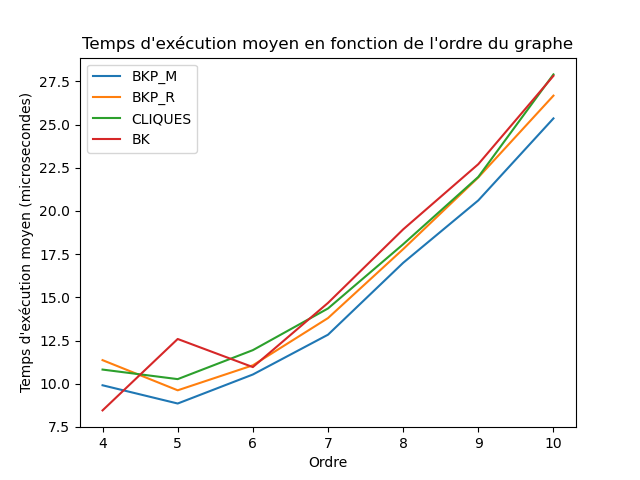
\includegraphics[width=\textwidth]{images/total_plot.png}
        \caption{}
        \label{fig:total_plot}
    \end{subfigure}
    \hfill
    \begin{subfigure}[b]{0.49\textwidth}
        \centering
        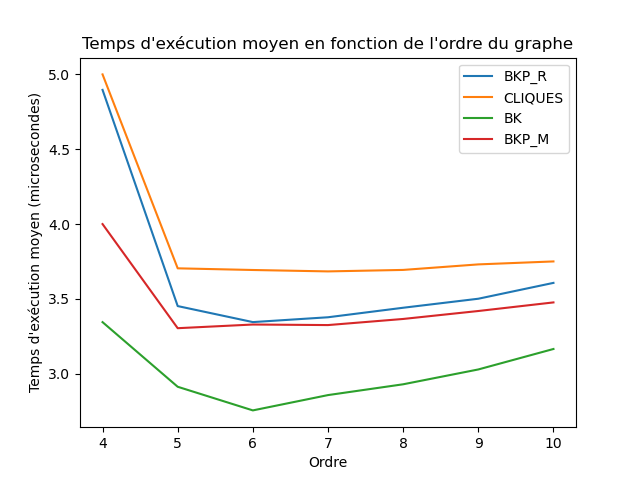
\includegraphics[width=\textwidth]{images/delay_plot.png}
        \caption{}
        \label{fig:delay_plot}
    \end{subfigure}
    \caption{Résultats des temps d'exécution pour différents algorithmes d'énumération des cliques maximales}
    \label{fig:res1}
\end{figure}

Nous pouvons constater en regardant le graphique \ref{fig:total_plot} que, clairement, les différents algorithmes d'énumération de cliques présentés suivent bien une complexité en temps exponetiel par rapport à l'ordre du graphe.

De plus, le graphique \ref{fig:delay_plot} nous montre une temps relativement constant entre l'énumération de chaque clique. Nous pouvons observé un temps moyen pour énumérer les cliques maximales plus élevé pour les graphes d'ordre 4.

En observant les temps obtenu pour les différents algorithmes, nous constatons que \texttt{BKP\_M} (avec pour pivot le noeud de degré maximum) semble se comporter mieux de manière générale.

L'analyse de ces résultats est cohérente avec les discussions théoriques présentées dans l'article \cite{CONTE20221}. L'efficacité des différents algorithmes dépend fortement de leurs approches spécifiques pour traiter les graphes, et la sélection de l'algorithme optimal peut varier en fonction des caractéristiques spécifiques du graphe à traiter.

Afin d'étayer ce dernier propos, nous allons présenter les mêmes tests mais en nous intéressants à des types de graphes particuliers :
\begin{itemize}
  \item Les graphes complets
  \item Les graphes vides
  \item Les graphes de Moon-Moser
\end{itemize}
Pour rappel, les graphes complets d'ordre \emph{n} n'ont qu'une et une seule clique maximales de taille \emph{n}, les graphes vides d'ordre \emph{n} possèdent \emph{n} cliques maximales de taille 1 et enfin, les graphes de Moon-Moser possèdent \(3^{n/3}\) cliques maximales (voir section \ref{subsec:graphes}).

La méthode de test reste la même. L'algorithme sans pivot \texttt{BK} à néansmoins dû être retiré des tests car celui-ci prenait trop de temps d'exécution.

\begin{figure}[ht]
  \centering
  \begin{subfigure}[b]{0.32\textwidth}
    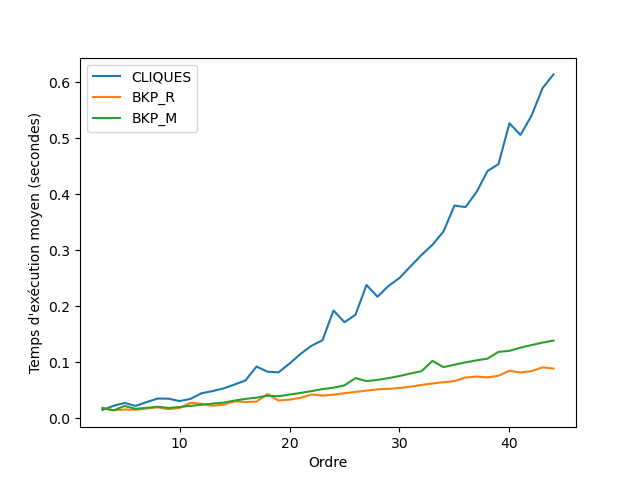
\includegraphics[width=\textwidth]{images/total_pivot_complete_plot.png}
    \caption{Complets}
    \label{subfig:total_complete}
  \end{subfigure}
  \begin{subfigure}[b]{0.32\textwidth}
    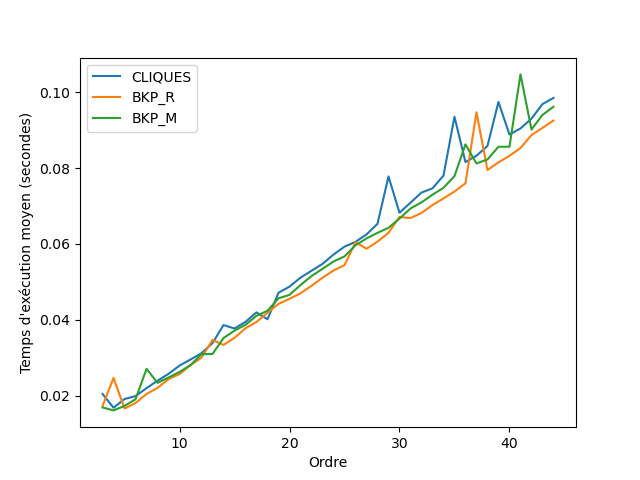
\includegraphics[width=\textwidth]{images/total_pivot_empty_plot.png}
    \caption{Vides}
    \label{subfig:total_empty}
  \end{subfigure}
  \begin{subfigure}[b]{0.32\textwidth}
    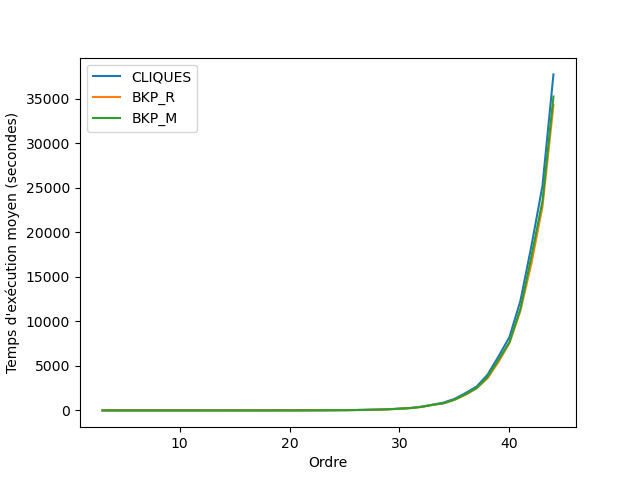
\includegraphics[width=\textwidth]{images/total_pivot_turan_plot.png}
    \caption{Moon-Moser}
    \label{subfig:total_turan}
  \end{subfigure}
  \caption{Temps d'exécution total pour énumérer toutes les cliques maximales}
  \label{fig:special_total}
\end{figure}

\begin{figure}[ht]
  \centering
  \begin{subfigure}[b]{0.32\textwidth}
    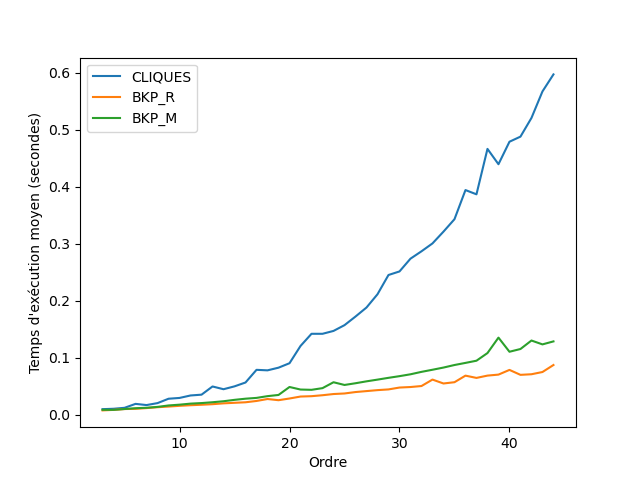
\includegraphics[width=\textwidth]{images/delay_pivot_complete_plot.png}
    \caption{Complets}
    \label{subfig:delay_complete}
  \end{subfigure}
  \begin{subfigure}[b]{0.32\textwidth}
    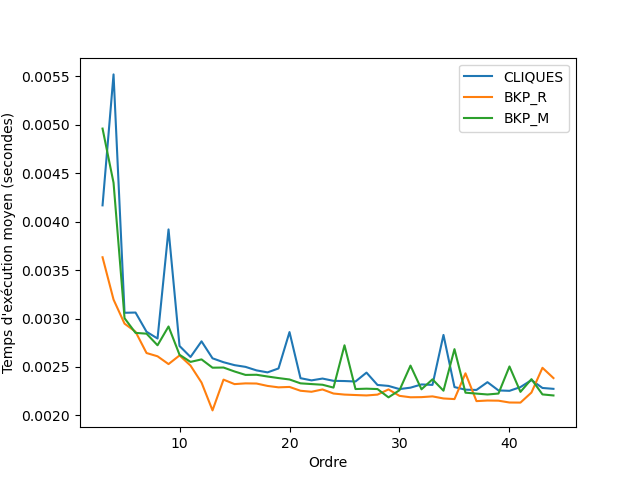
\includegraphics[width=\textwidth]{images/delay_pivot_empty_plot.png}
    \caption{Vides}
    \label{subfig:delay_empty}
  \end{subfigure}
  \begin{subfigure}[b]{0.32\textwidth}
    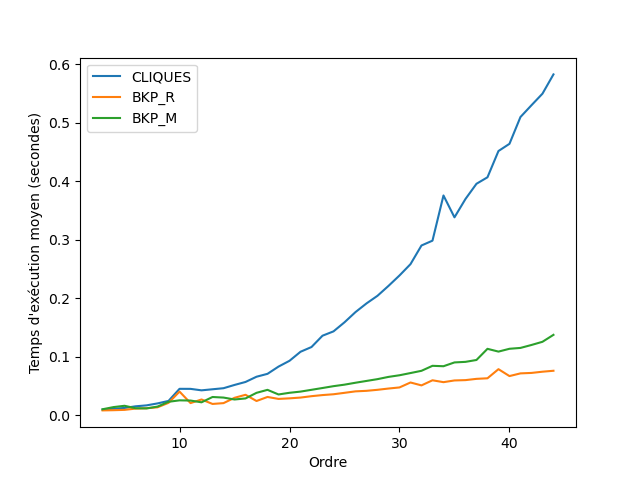
\includegraphics[width=\textwidth]{images/delay_pivot_turan_plot.png}
    \caption{Moon-Moser}
    \label{subfig:delay_turan}
  \end{subfigure}
  \caption{Délais entre chaque énumération de clique maximale}
  \label{fig:special_delay}
\end{figure}


% TODO: explication correcte pour les résultats
% TODO: un tableau avec des graphes classiques et comparer avec un tableau avec des graphes complets et un autre avec des graphes de Turan pour voir

\section{Conclusion}

% TODO

\bibliographystyle{abbrv}
\bibliography{biblio}

\end{document}

%%% Local Variables:
%%% mode: latex
%%% TeX-master: t
%%% End:
